\documentclass[11pt]{article}
\usepackage[letterpaper,margin=0.7in]{geometry}
\usepackage[T1]{fontenc}
\usepackage{lmodern,microtype,amsmath,amssymb,graphicx,subcaption,float,booktabs,listings}
\usepackage[section]{placeins}
\usepackage{xcolor,hyperref}
\hypersetup{pdftitle={Computational Photography HW5},pdfauthor={Chung-Ting Tsai},colorlinks=true,linkcolor=blue!45!black,urlcolor=blue!45!black}
\graphicspath{{figures/}}
\captionsetup{font=small,labelfont=bf,skip=6pt}
\setlength{\parindent}{0pt}
\setlength{\parskip}{6pt}
\setlength{\textfloatsep}{12pt plus 2pt minus 2pt}
\setlength{\intextsep}{10pt plus 2pt minus 2pt}
\lstset{basicstyle=\ttfamily\small,breaklines=true,frame=single,rulecolor=\color{black!20},backgroundcolor=\color{black!3},aboveskip=6pt,belowskip=6pt}
\newcommand{\fig}[4]{\begin{figure}[H]\centering\includegraphics[width=#2\linewidth,height=0.29\textheight,keepaspectratio]{#1}\caption{#3}\label{#4}\end{figure}}
\begin{document}
\begin{center}
{\Large\bfseries 15-663 Computational Photography}\\[4pt]
{\large Homework 5: Photometric Stereo}\\[4pt]
Chung-Ting Tsai
\end{center}

\section{Photometric stereo}
\subsection*{Linear ambiguity}
I use the non-diagonal transformation
\[
Q=\begin{bmatrix}1&0&0\\0&1&0\\0&-1&1\end{bmatrix},\qquad
L_Q=Q\widetilde L,\qquad B_Q=Q^{-T}\widetilde B.
\]
The two sets of albedos and normals look different, but their image predictions are identical: $L_Q^TB_Q=\widetilde L^T\widetilde B$. This shows why a good image fit alone does not determine the correct surface.
\fig{face_svd.png}{1}{SVD albedo and normals, and their counterparts after applying $Q^{-T}$. A common reflection of the $z$ component is applied to the displayed normals in both cases, consistent with the later orthographic reconstruction. Normal maps show the full image without masking the background.}{fig:svd}

\subsection*{Enforcing integrability}
I enforce integrability following Yuille and Snow~\cite{yuille}, with Gaussian smoothing applied only when computing the pseudo-normal derivatives. I then flip the third component to resolve the concave/convex branch, as suggested in the assignment.

\subsection*{Discussion}
\begin{itemize}\setlength{\itemsep}{2pt}
\item \textbf{Choice of smoothing.} I tested $\sigma\in\{1,2,4,8,12,20\}$ (Figures~\ref{fig:sigma} and~\ref{fig:sigma-albedo}) and use $\sigma=8$ for the supplied face. Small kernels leave more fine-scale variation in the recovered field; large kernels change the inferred transformation because the derivatives mix increasingly distant surface regions. This parameter affects the global ambiguity estimate, not just local noise.
\item \textbf{Remaining ambiguity.} Enforcing integrability gives a recognizable face, but it does not fix its depth scale and tilt. The remaining three degrees of freedom correspond to generalized bas-relief (GBR) transformations~\cite{belhumeur}.
\end{itemize}
\fig{sigma_sweep.png}{0.9}{Integrability-corrected normals for six Gaussian standard deviations. Only the derivative calculation uses the smoothed pseudo-normal image. All panels use the same RGB normal encoding, without a background mask.}{fig:sigma}

\fig{sigma_albedo_sweep.png}{0.9}{Recovered albedo for the same six Gaussian standard deviations as the normal-map sweep. Each panel is normalized independently for display.}{fig:sigma-albedo}

\clearpage
\subsection*{Normal integration and manual GBR}
For a height field with normal proportional to $(-z_x,-z_y,1)$, I compute
\[
p=z_x=-n_x/d,\qquad q=z_y=-n_y/d,\qquad
d=\operatorname{sgn}_{+}(n_z)\max(|n_z|,0.05),
\]
where $\operatorname{sgn}_{+}(0)=1$. The denominator floor avoids unstable division near grazing normals; it is a numerical safeguard that can change the reconstructed slopes. I test both supplied integration functions on the same slopes. For the face comparisons I use Poisson integration, since it avoids the periodic continuation implicit in the Fourier approach. Background slopes are zero in this rectangular-domain experiment; the depth maps in the normal integration results show the full image, including the background. In depth images, black denotes the front and white denotes farther regions.

I test GBR parameters $(\mu,\nu,\lambda)\in\{(0,0,0.5),(0,0,1),(0,0,2),(0.2,0,2),(0,0.2,2)\}$, using the assignment's convention $B_G=G^{-T}B_{\mathrm{int}}$. I keep $(0,0,2)$ as a simple visual choice: it changes the relief without adding a global tilt. This is a manual choice, not a calibrated estimate of the true shape.
\fig{face_gbr_normals.png}{1}{GBR experiments after enforcing integrability. Changing $\lambda$ changes the normal tilts and relief; nonzero $\mu$ or $\nu$ adds a tilt.}{fig:gbr}

\clearpage
\subsection*{Normal integration: depth maps and surfaces}
Figure~\ref{fig:integration-depth} shows the integrated depth before and after the selected GBR, including both integration methods. Figure~\ref{fig:integration-surfaces} shows two views of each Poisson-reconstructed surface.
\begin{figure}[H]
\centering
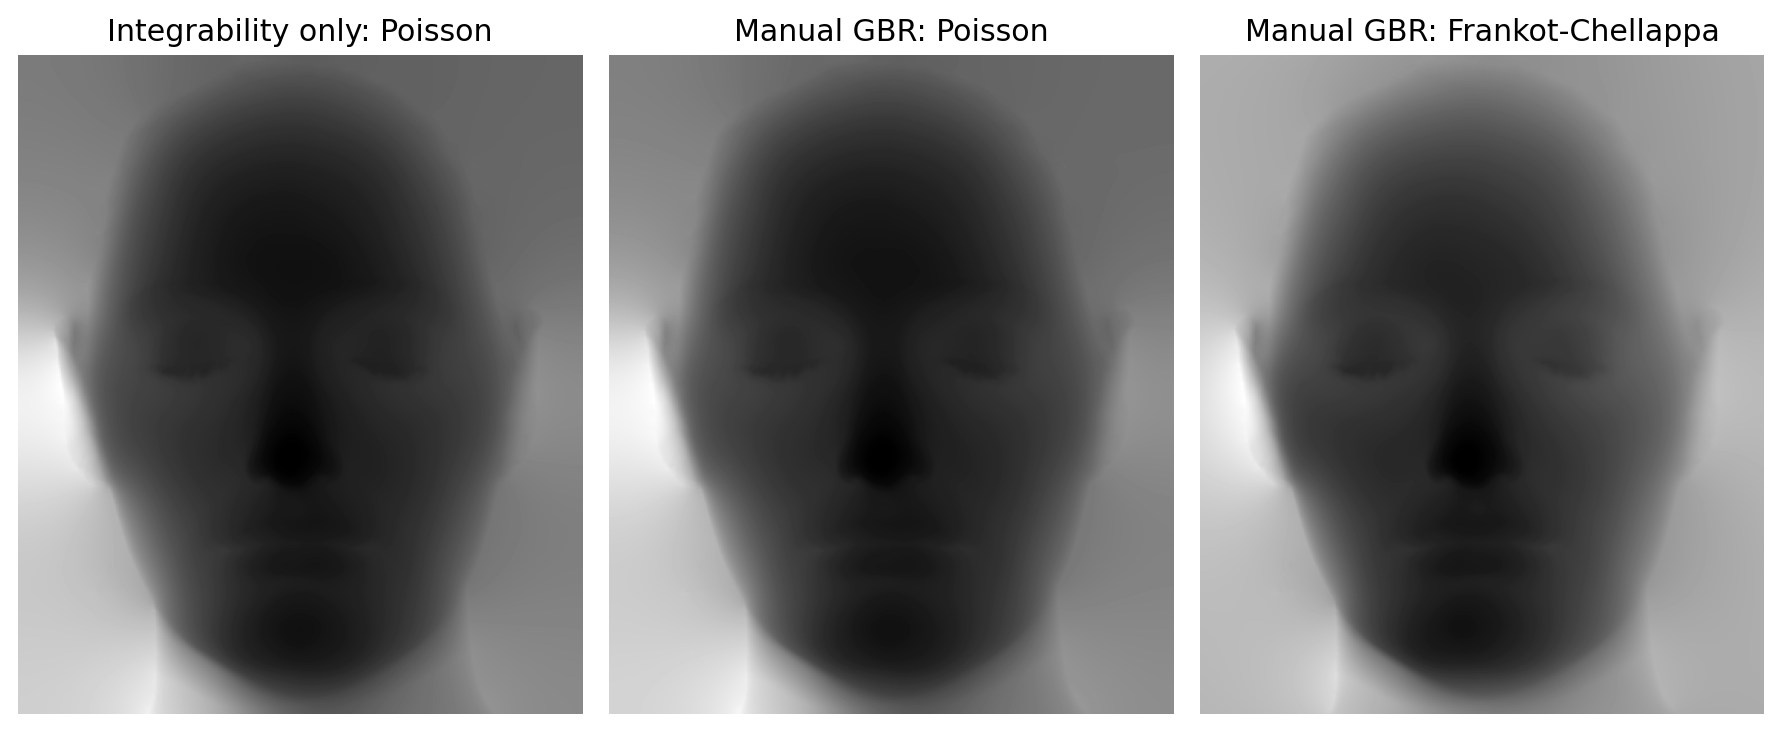
\includegraphics[width=0.95\linewidth,height=2.8in,keepaspectratio]{integration_uncalibrated.png}
\caption{Depth maps after enforcing integrability: Poisson integration before manual GBR, and Poisson and Frankot--Chellappa integration after applying $(\mu,\nu,\lambda)=(0,0,2)$. The full depth image is displayed without a foreground mask. Depth brightness is normalized independently in each panel, with black at the front and white farther away.}
\label{fig:integration-depth}
\end{figure}
\begin{figure}[H]
\centering
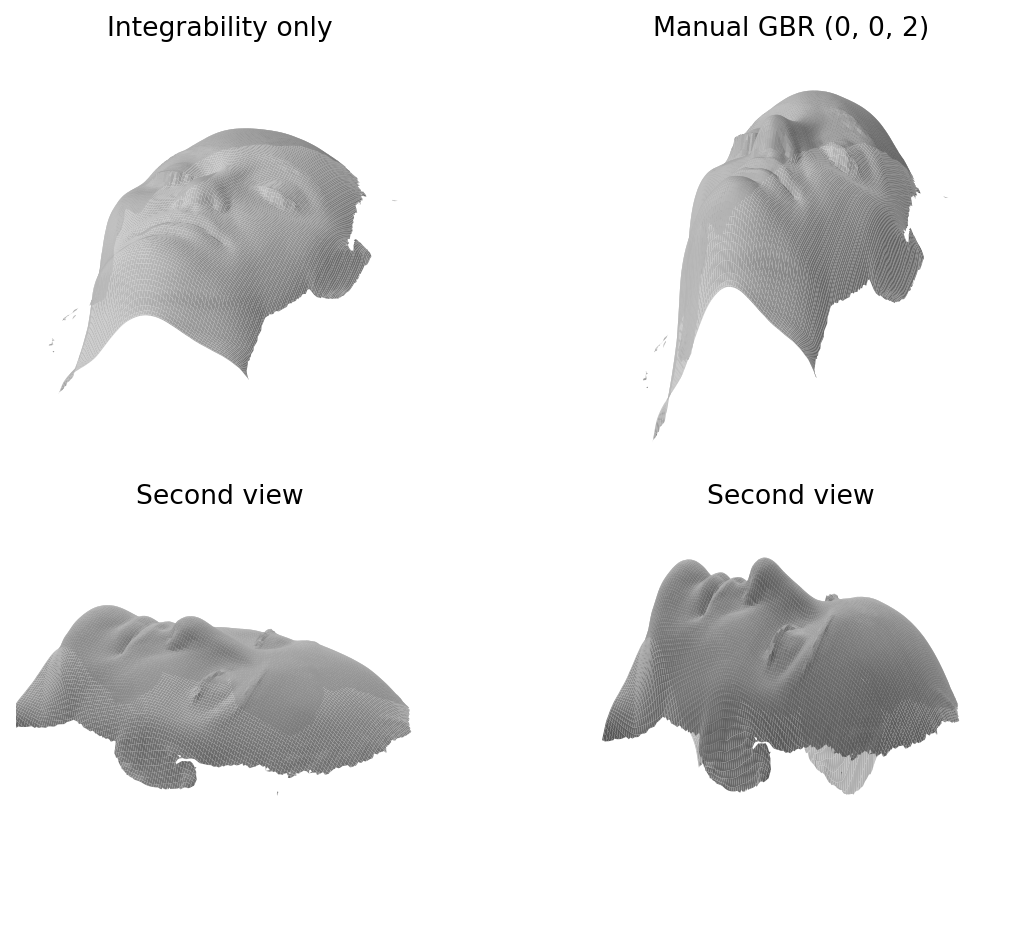
\includegraphics[width=0.91\linewidth,height=4.6in,keepaspectratio]{integration_surfaces.png}
\caption{Two views of the Poisson-integrated surface before and after the selected manual GBR. The transform changes the face's relief. The plots use independent height-axis ranges and do not determine a metric depth scale.}
\label{fig:integration-surfaces}
\end{figure}

\clearpage
\subsection*{Calibrated photometric stereo}
I load the seven light vectors using \texttt{load\_sources}, which returns the $7\times3$ matrix $S=L^T$. I solve all pixel systems together with
\[
B_{\mathrm{cal}}=\underset{B}{\arg\min}\,\|SB-I\|_F^2
=\texttt{numpy.linalg.lstsq}(S,I).
\]
I normalize its columns for albedo and normals, apply the same $z$-axis display reflection, and integrate using the same orthographic convention. The relative intensity residual $\|SB_{\mathrm{cal}}-I\|_F/\|I\|_F$ is 4.61\%.

\textbf{Comparison.} Both methods recover the eyes, nose, lips and chin. Calibration fixes the linear lighting ambiguity directly and avoids having to choose a GBR by appearance. The uncalibrated face has similar detail, but its relief and tilt remain uncertain; the manual GBR changes these without adding new evidence. The known-light result is a reference obtained under the Lambertian model, not ground-truth depth.
\fig{face_comparison.png}{0.81}{Albedo and normals after integrability, after the selected manual GBR, and with known lighting. The third row compares manual-GBR Poisson depth, manual-GBR Frankot--Chellappa depth, and calibrated Poisson depth, including the background without masking. Albedo and depth panels are normalized independently for display.}{fig:calibrated}
\fig{face_surfaces.png}{0.91}{Two views of the integrability-only, manually transformed and calibrated surfaces. Each plot has its own height-axis range; absolute scale cannot be inferred by comparing apparent plot heights.}{fig:surfaces}

\clearpage
\section{Capture and reconstruct my own shapes}
\subsection*{Capture and preprocessing}
I captured seven NEF images of a ceramic cup and seven of a boot, keeping the view fixed while varying illumination. The boot is the more diffuse example, although its collar, eyelets and sole are not perfectly Lambertian. The glazed cup is the example that violates the assumptions through glossiness and the concavity around its handle. The EXIF settings are summarized in Table~\ref{tab:capture}; camera distance and light directions were not measured.

I decode the RAW files using \texttt{dcraw -4 -h -r 1 1 1 1 -o 1}: linear 16-bit sRGB, half-size demosaicing and fixed unit white-balance multipliers. Automatic brightness normalization is disabled. The green cast in the input displays comes from these fixed multipliers; it is not corrected separately in each frame. Luminance estimation uses the linear data, whereas input photographs are gamma-encoded for display.

\subsection*{Segmentation and reconstruction}
\begin{enumerate}\setlength{\itemsep}{2pt}
\item \textbf{Object mask.} I form a maximum-over-light RGB composite, seed each object's silhouette with a polygon, and refine a band around that polygon using seven GrabCut iterations. The largest foreground component is retained. The cup handle's hole is excluded. The same mask is used for every image; these are capture-specific masks, not a general semantic segmentation model.
\item \textbf{Masked fitting.} I set the background to zero before rank-3 SVD. Integrability uses $\sigma=2$, a six-pixel erosion to avoid derivatives across the silhouette, and rejection of the largest 10\% of relative rank-3 residuals. Albedo and normals are estimated on the segmented object.
\item \textbf{Masked integration.} I solve a sparse least-squares problem for the differences of neighboring foreground depths. Only edges whose endpoints are both inside the mask contribute. Each connected component has one arbitrary depth anchor; the background and handle hole impose no artificial zero-gradient constraints. Orthographic slopes use $|n_z|\geq0.1$ in the denominator.
\item \textbf{Novel lighting.} I render $R=a\max(0,n\cdot\ell)$ with $\ell=(-0.358,-0.268,0.894)$ in the reconstruction coordinates. These renderings use the integrability-only estimates; they do not simulate cast shadows, specular reflections or interreflections.
\end{enumerate}
\begin{table}[H]\centering\small
\begin{tabular}{lll}\toprule
Setting & Cup & Boot \\\midrule
Images & 7 RAW NEFs & 7 RAW NEFs \\
Focal length / aperture / ISO & 55\,mm / $f/5.6$ / 100 & 55\,mm / $f/5.6$ / 100 \\
Exposure time & 4\,s & 8\,s \\
Processed object crop ($H\times W$) & $320\times380$ & $440\times810$ \\
Foreground pixels & 64691 & 182436 \\
Median relative rank-3 residual & 5.28\% & 3.74\% \\
Rank-3 explained intensity energy & 98.93\% & 99.69\% \\\bottomrule
\end{tabular}\caption{Capture settings and photometric diagnostics. The full image is resized to width 2000 before taking the object crop. Residuals measure intensity fit, not depth accuracy.}\label{tab:capture}\end{table}

\clearpage
\subsection*{Cup: results and discussion}
The segmentation separates the cup from the desk and removes the handle hole. The cup's glossy surface violates the Lambertian reflectance assumption: specular highlights change with the lighting direction, so the algorithm can mistake these intensity changes for changes in surface orientation. This likely contributes to the strong vertical transition near the highlight in the normal map and the folded, tilted reconstruction instead of a clean cylinder. Additional artifacts appear around the printed logo. Masking prevents the background from controlling the solve, but cannot remove these reflectance effects.

The relighting produces a new shading pattern, but its sharp transitions inherit the errors in the recovered normals. It should be interpreted as a rendering of the estimated field rather than a prediction validated against another photograph.
\fig{cup_baseline.png}{0.95}{Cup input, shared segmentation, integrability-only albedo, normals and depth, and rendering under the new directional light. Depth brightness is normalized, with black at the front and white farther away. The captured image is gamma-encoded for display; reconstruction uses linear luminance.}{fig:cup}
\fig{cup_surface_baseline.png}{0.7}{Cup surface after enforcing integrability. The folded shape reflects the errors in the recovered normal field.}{fig:cup-surface}

\clearpage
\subsection*{Boot: results and discussion}
The boot gives a lower photometric residual than the cup, and its normal map contains recognizable changes along the upper, toe and sole. The tongue, laces, collar and eyelets introduce shadows, occlusion and reflectance changes, so this object is only approximately diffuse.

The reconstructed depth still has a strong global tilt and spurious relief. The low rank-3 residual therefore does not imply a correct shape. The novel-light rendering preserves the outline and some local structure, but its shading is affected by the same normal errors. I retain the untransformed integrable estimate as the Part~2 baseline and compare automatic GBR recovery separately below; a manual GBR cannot by itself resolve the local artifacts.
\fig{shoes_baseline.png}{0.98}{Boot input, segmentation, integrability-only albedo, normals and depth, and novel-light Lambertian rendering. Pixels outside the object are excluded from fitting and integration.}{fig:boot}
\fig{shoes_surface_baseline.png}{0.9}{Boot surface after enforcing integrability, viewed at elevation $55^\circ$ and azimuth $-90^\circ$ to show its outline and local relief. The horizontal aspect ratio follows the image dimensions; vertical display scale is chosen for visibility and is not metric.}{fig:boot-surface}

\clearpage
\section{Bonus: Resolving the GBR ambiguity by entropy minimization}
\subsection*{Implementation}
I implement the albedo-entropy search of Alldrin, Mallick and Kriegman~\cite{entropy}. Starting from integrable pseudo-normals, the algorithm favors the GBR whose albedos have a concentrated histogram. With columns used for pseudo-normals, my implementation uses the paper's recovery parameterization
\[
B_{\mathrm{after}}=G^TB_{\mathrm{before}},\qquad
H(a)=-\sum_j p_j\log p_j.
\]
This differs from the assignment's forward ambiguity convention $G^{-T}B$: the two parameter triples must not be compared without inverting the transform. The histogram has 256 bins over each candidate's own albedo range, and its support is recomputed per candidate.

I use a fixed entropy mask, excluding silhouette pixels and the highest 10\% of rank-3 residuals and image-gradient magnitudes. I search $\mu,\nu\in[-5,5]$ and $\lambda\in[0.01,5]$ with coarse-to-fine grids. The face uses $9^3$ candidates per level for five levels and all 86842 inliers. Each captured object uses $7^3$ candidates per level for four levels on 12000 fixed random inliers. The implementation uses ordinary SVD; it omits the paper's visibility-weighted missing-data preprocessing.

\subsection*{Supplied face}
The selected parameters are $(\mu,\nu,\lambda)=(-0.0195,0.0342,0.5168)$, and the discrete entropy decreases from 5.1174 to 4.3159 nats. The albedo becomes less variable and the face remains recognizable. This criterion provides an automatic GBR choice, but it does not prove recovery of the physical surface or resolve the concave/convex branch.
\fig{face_entropy.png}{0.84}{Face before and after entropy minimization. The depth and surface panels show the corrected result; albedo and normal panels compare the two estimates.}{fig:face-entropy}

\clearpage
\subsection*{Captured objects: comparison}
For the cup the search returns $(-0.7407,0.3086,0.3950)$. For the boot, the selected parameters are reported in the reproducibility files and summarized below. The cup logo, glaze and unglazed base, and the boot's multiple materials, weaken the few-albedo-values prior. Entropy recovery changes the global relief, but leaves local artifacts in both objects.
\begin{table}[H]\centering\small
\begin{tabular}{lrrr}\toprule
Object & $\mu$ & $\nu$ & $\lambda$ \\\midrule
Cup & -0.7407 & 0.3086 & 0.3950 \\
Boot & -0.9259 & 0.6790 & 0.6877 \\\bottomrule
\end{tabular}\caption{Selected entropy parameters, using $B_{\mathrm{after}}=G^TB_{\mathrm{before}}$. These are not the manual inverse-transpose parameters of Part~1.}\end{table}
\fig{cup_entropy.png}{0.85}{Cup: segmentation, corrected normals, relative rank-3 residual, depths before and after correction, and the corrected surface. The residual map uses its own color scale.}{fig:cup-entropy}
\fig{shoes_entropy.png}{0.85}{Boot: corresponding entropy-recovery outputs. Local seams and grazing normals still produce spurious relief. Independent depth color scales and surface axes prevent metric comparisons.}{fig:boot-entropy}

\clearpage
\subsection*{Albedo distributions before and after entropy recovery}
Figure~\ref{fig:albedo-distributions} compares the albedo distributions for the face, cup and boot. Each before/after pair uses exactly the same pixels as its entropy search: all selected face inliers, and the fixed 12000-pixel samples for the captured objects. The histograms use 256 bins over each candidate's own albedo range, matching the implemented objective. Bar heights are fractions of the sampled pixels, and the vertical scale is shared within each pair. Albedo units and horizontal ranges are arbitrary, so concentration and entropy should be compared rather than absolute albedo values.

The selected GBR reduces histogram entropy in all three cases. A more concentrated histogram is consistent with the search objective, but does not by itself establish a correct surface, especially for the glossy cup and the boot's multiple materials.
\begin{figure}[H]
\centering
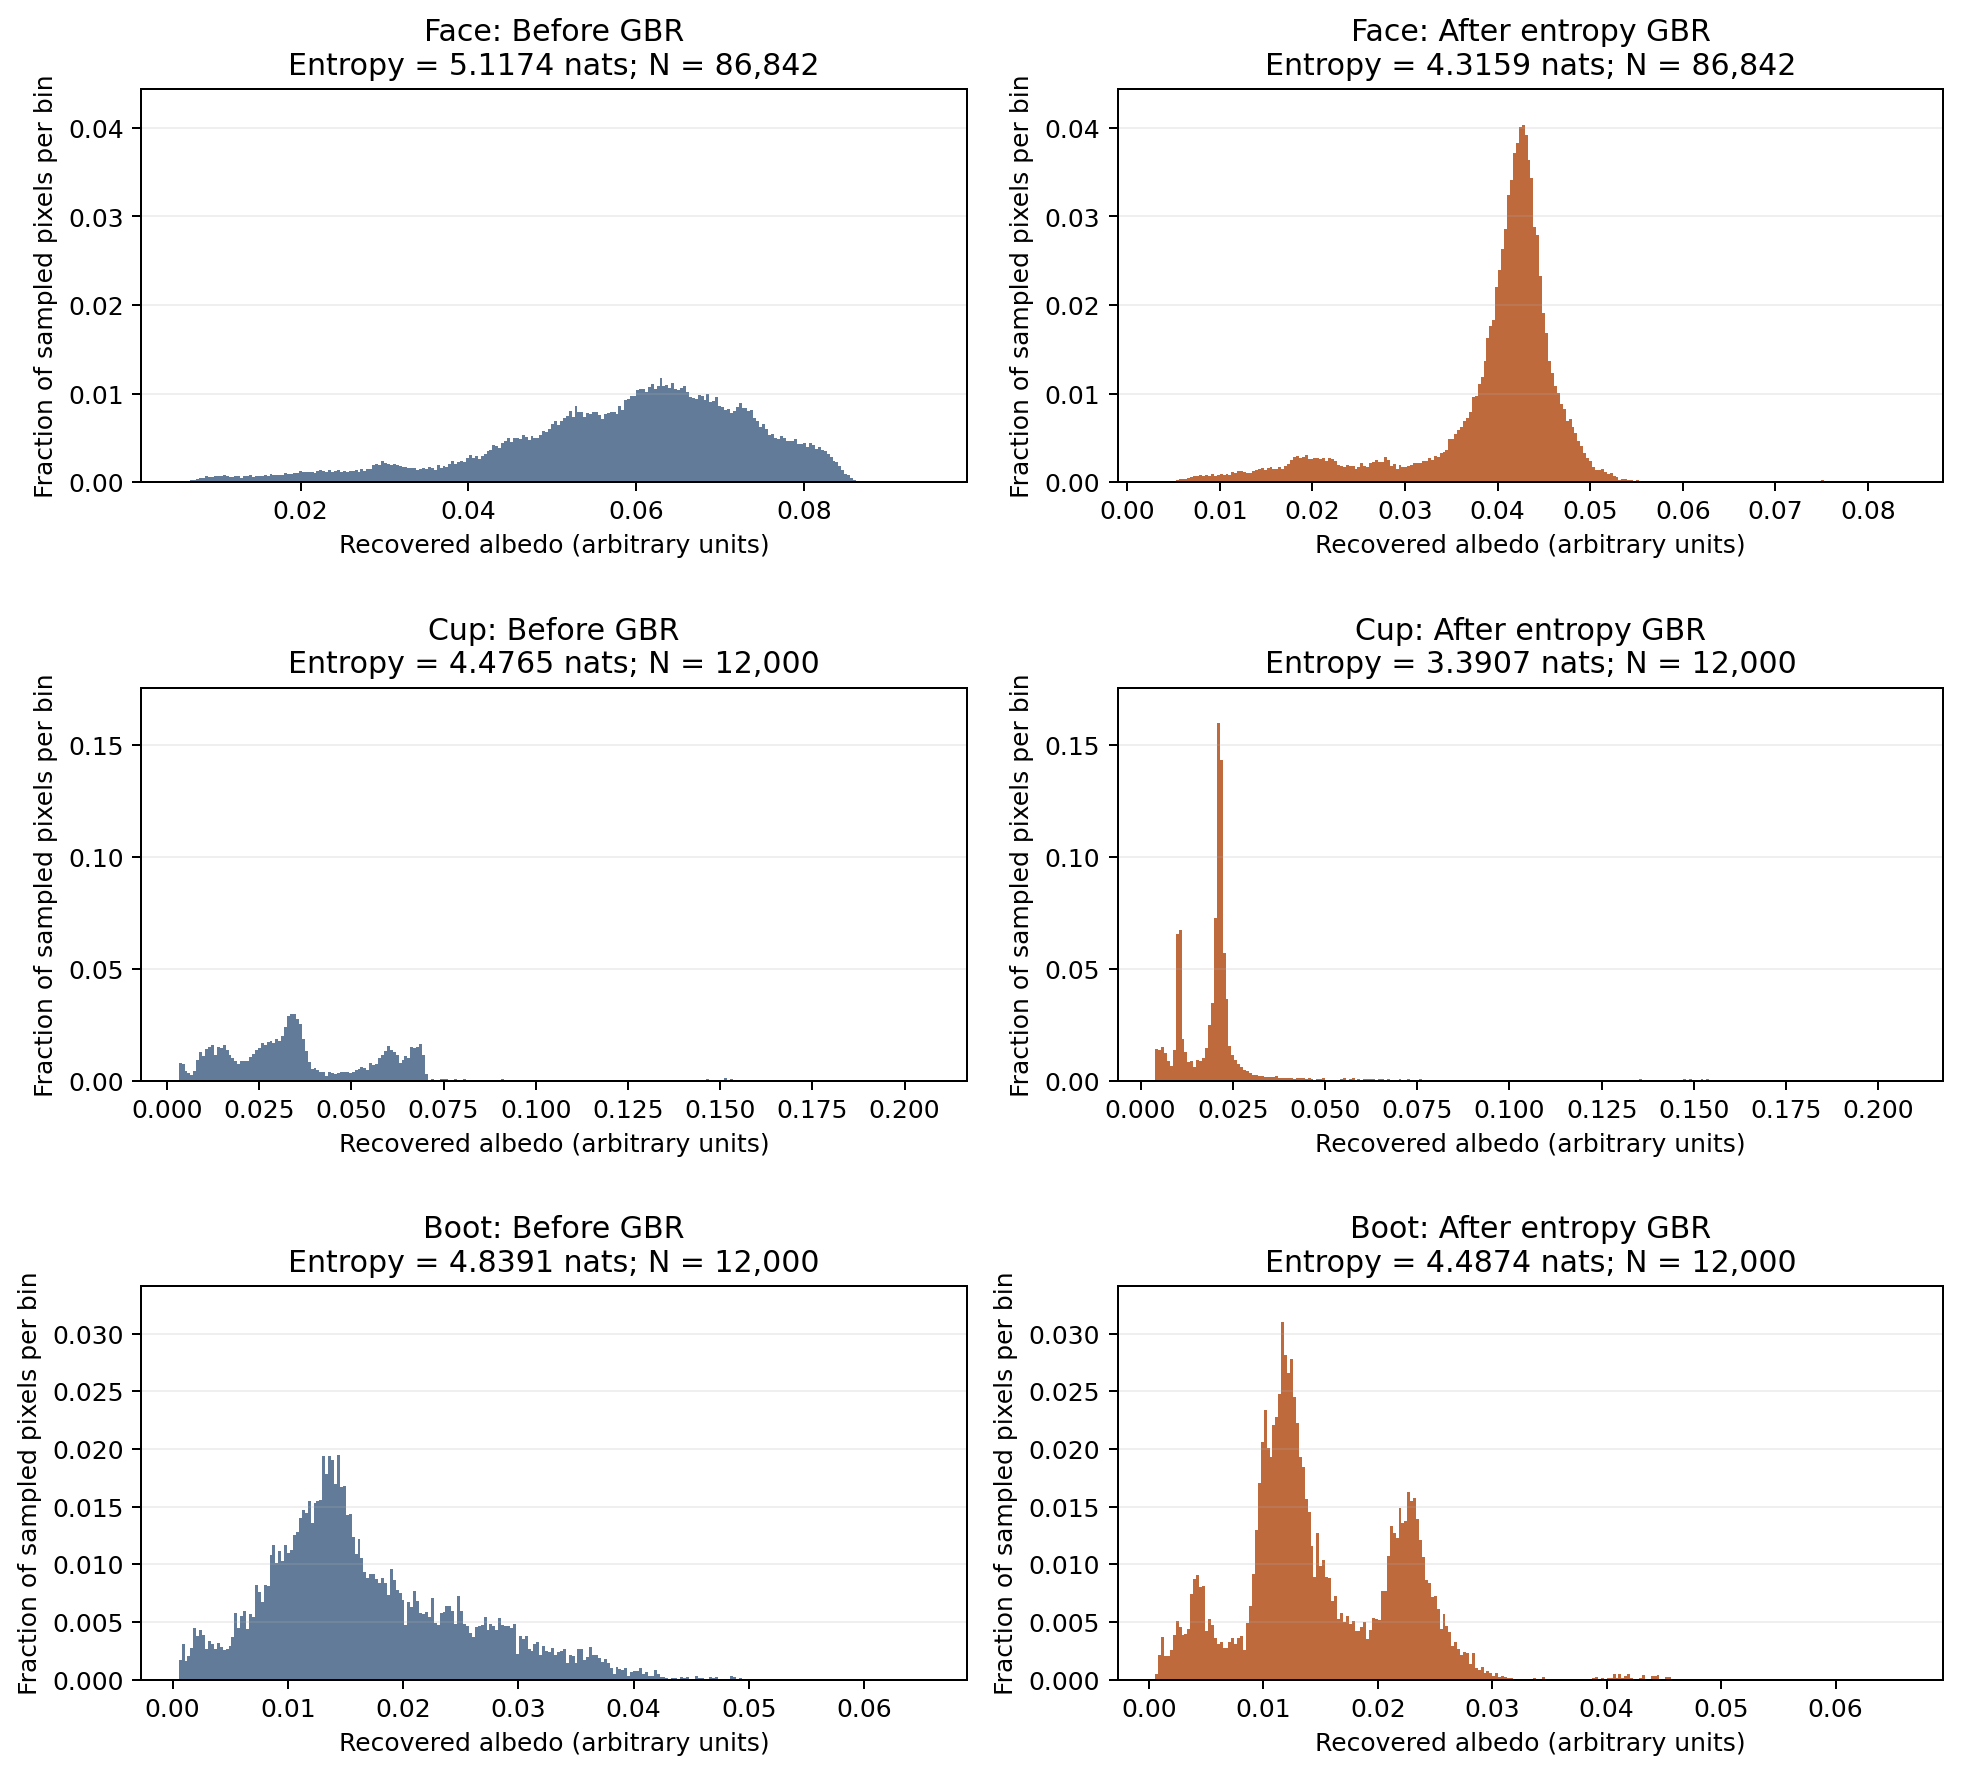
\includegraphics[width=\linewidth,height=6.7in,keepaspectratio]{albedo_distributions.png}
\caption{Albedo distributions before (left) and after entropy-based GBR recovery (right). Rows show the supplied face, cup and boot. Each panel reports discrete entropy in nats and the number of sampled pixels. Bin edges are recomputed for each candidate, as in the entropy search; y-axes show probability per bin rather than probability density.}
\label{fig:albedo-distributions}
\end{figure}

\clearpage
\subsection*{Entropy GBR: surface comparisons}
These comparisons show how entropy minimization changes the reconstructed surfaces. Both estimates remain distorted; the change in appearance does not establish geometric accuracy.
\fig{cup_surfaces.png}{0.9}{Cup surfaces before and after entropy-based GBR recovery. Independent plotting scales do not provide a metric comparison of relief.}{fig:cup-entropy-surfaces}
\fig{shoes_surfaces.png}{0.95}{Boot surfaces before and after entropy-based GBR recovery, both viewed at elevation $55^\circ$ and azimuth $-90^\circ$. The same display aspect is used for both; vertical scale remains arbitrary.}{fig:boot-entropy-surfaces}

\clearpage
\section{Bonus: Using a perspective camera}
\subsection*{Implementation}
I implement the linear perspective integrability formulation of Papadhimitri and Favaro~\cite{perspective}. From the rank-3 pseudo-normals and their smoothed derivatives, I construct a matrix with one row and nine coefficients per fitted pixel. If $u,v$ are coordinates relative to the principal point and $f$ is the focal length in pixels, the row contains the three blocks
\[
\left[\;(B_u\times B)^T,\ (B_v\times B)^T,
-\frac{u}{f}(B_u\times B)^T-\frac{v}{f}(B_v\times B)^T\;\right].
\]
The smallest right singular vector is reshaped into the columns of $\Psi$, and I recover $\widehat B=\Psi^{-1}B$. A single global sign is chosen so that the median dot product between normals and viewing rays is positive. Unlike the orthographic display convention, no individual normal channel is flipped here.

For axial camera distance $d$ (the third coordinate before choosing its global scale), I integrate log-distance gradients
\[
\partial_u\log d=\frac{-n_x}{un_x+vn_y+fn_z},\qquad
\partial_v\log d=\frac{-n_y}{un_x+vn_y+fn_z},
\]
then set $d=\exp(g-\operatorname{median}(g))$. Points are $(ud/f,vd/f,d)$, up to a global scale. Near-grazing rays are excluded. The displayed results use masked, incidence-weighted integration with three Huber reweighting iterations.

\subsection*{Face: assumed intrinsics versus reference-assisted fitting}
The original $f=1$ result has nearly constant normals. Using known-light normal references on alternating $16$-pixel training blocks, I select $\sigma=8$, six-pixel fitting-mask erosion, $(c_x,c_y)=(184,310)$ and effective $f=1318.74$ after focal/normal rescaling. Mean angular error is $4.58^\circ$ on training blocks and $4.56^\circ$ on held-out blocks.

\textbf{This is reference-assisted fitting, not independent camera calibration.} I integrate foreground log-depth with incidence weights and three Huber reweighting iterations, an extension to the paper's solver. The face depth is cleaner, with remaining edge artifacts and scale distortion. Cup and boot results use the same updated integration but retain their original perspective normals.

\fig{perspective_normals.png}{1}{Original perspective normals, reference-assisted fitted normals, and the known-light normal reference. These panels use the perspective sign convention, which differs from the orthographic normal displays.}{fig:perspective-normals}

\clearpage
\subsection*{Perspective results and limitations}
For my captures, I approximate $f_{\rm px}=(55/23.5)\times2000=4680.85$ pixels using a 23.5\,mm sensor width and shift the assumed full-frame center by each crop offset. This gives $(c_x,c_y)=(530,-183.33)$ for the cup and $(590,36.67)$ for the boot. A principal point outside the crop is possible because both objects lie below the center of the full image. These are approximate intrinsics; lens distortion is not calibrated.

The ratio of the second-smallest to smallest constraint singular values is 2.37 for the cup and 1.24 for the boot. In particular, the boot has little separation of the putative null direction. Both surfaces are unstable, consistent with using a long focal length to capture an approximately orthographic view. I do not interpret the perspective outputs as successful metric reconstructions.
\textbf{Why normals can look reasonable while depth fails.} Normal colors encode bounded, local directions, but perspective integration divides by $un_x+vn_y+fn_z$. Small errors become large gradients when this denominator approaches zero. Spatially inconsistent gradient errors accumulate during integration, and exponentiating the integrated log-distance amplifies them further. Approximate intrinsics and weak perspective constraints can therefore produce plausible-looking normal maps without a stable surface.

\begingroup
\renewcommand{\fig}[4]{\begin{figure}[H]\centering\includegraphics[width=#2\linewidth,height=1.3in,keepaspectratio]{#1}\caption{#3}\label{#4}\end{figure}}
\fig{perspective_face.png}{0.73}{Face: updated reference-assisted albedo and normals with robust weighted perspective depth. Depth is shown over its 1--99\% display range; the underlying depth values are not clipped.}{fig:perspective-face}
\fig{cup_perspective.png}{0.73}{Cup: perspective albedo and normals with updated robust weighted depth, using approximate capture intrinsics. Normal estimates are retained; depth artifacts remain.}{fig:perspective-cup}
\fig{shoes_perspective.png}{0.73}{Boot: perspective albedo and normals with updated robust weighted depth. Normal estimates are retained; weak nullspace separation and shadow/material violations still limit the result.}{fig:perspective-boot}
\endgroup

\clearpage
\begingroup\small
\begin{thebibliography}{5}
\bibitem{entropy} N. G. Alldrin, S. P. Mallick, and D. J. Kriegman. Resolving the generalized bas-relief ambiguity by entropy minimization. In \emph{CVPR}, 2007.
\bibitem{belhumeur} P. N. Belhumeur, D. J. Kriegman, and A. L. Yuille. The bas-relief ambiguity. \emph{International Journal of Computer Vision}, 35(1):33--44, 1999.
\bibitem{frankot} R. Frankot and R. Chellappa. A method for enforcing integrability in shape from shading algorithms. \emph{IEEE Transactions on Pattern Analysis and Machine Intelligence}, 10(4):439--451, 1988.
\bibitem{perspective} T. Papadhimitri and P. Favaro. A new perspective on uncalibrated photometric stereo. In \emph{CVPR}, pages 1474--1481, 2013.
\bibitem{yuille} A. Yuille and D. Snow. Shape and albedo from multiple images using integrability. In \emph{CVPR}, pages 158--164, 1997.
\end{thebibliography}
\endgroup

\subsection*{Acknowledgement}
The visualizations, numerical checks and writing of this report were prepared in collaboration with OpenAI Codex. The capture images and assignment implementation were provided by the author; the added preprocessing and evaluation code are included with the report.
\end{document}
